\documentclass[9pt]{beamer}

\input macros-Elaine.tex

\title{Higher-level rules for sequent calculus}
\author[Miller, Pimentel]{
	\emph{Dale Miller} \\ {\small \'Ecole Polytechnique, France} \\\ \\ 
	{\small Joint work with Elaine Pimentel}
}




\begin{document}

\begin{frame}
	\titlepage
\end{frame}	


\begin{frame}{The original axioms-as-rules problem}

\begin{overlayarea}{\textwidth}{7cm}	
\only<1->{	
	How to incorporate \emphdr{inference rules} encoding axioms into existing proof systems 
	
	for \emphdb{classical and intuitionistic logics}?
}

\only<2-3>{
\medskip

\emphdo{Gentzen:} Add mathematical theories to first-order logic.

\begin{center}
{\em Consistency of the arithmetic without complete induction.}
\end{center}

\begin{tabular}{lcl}
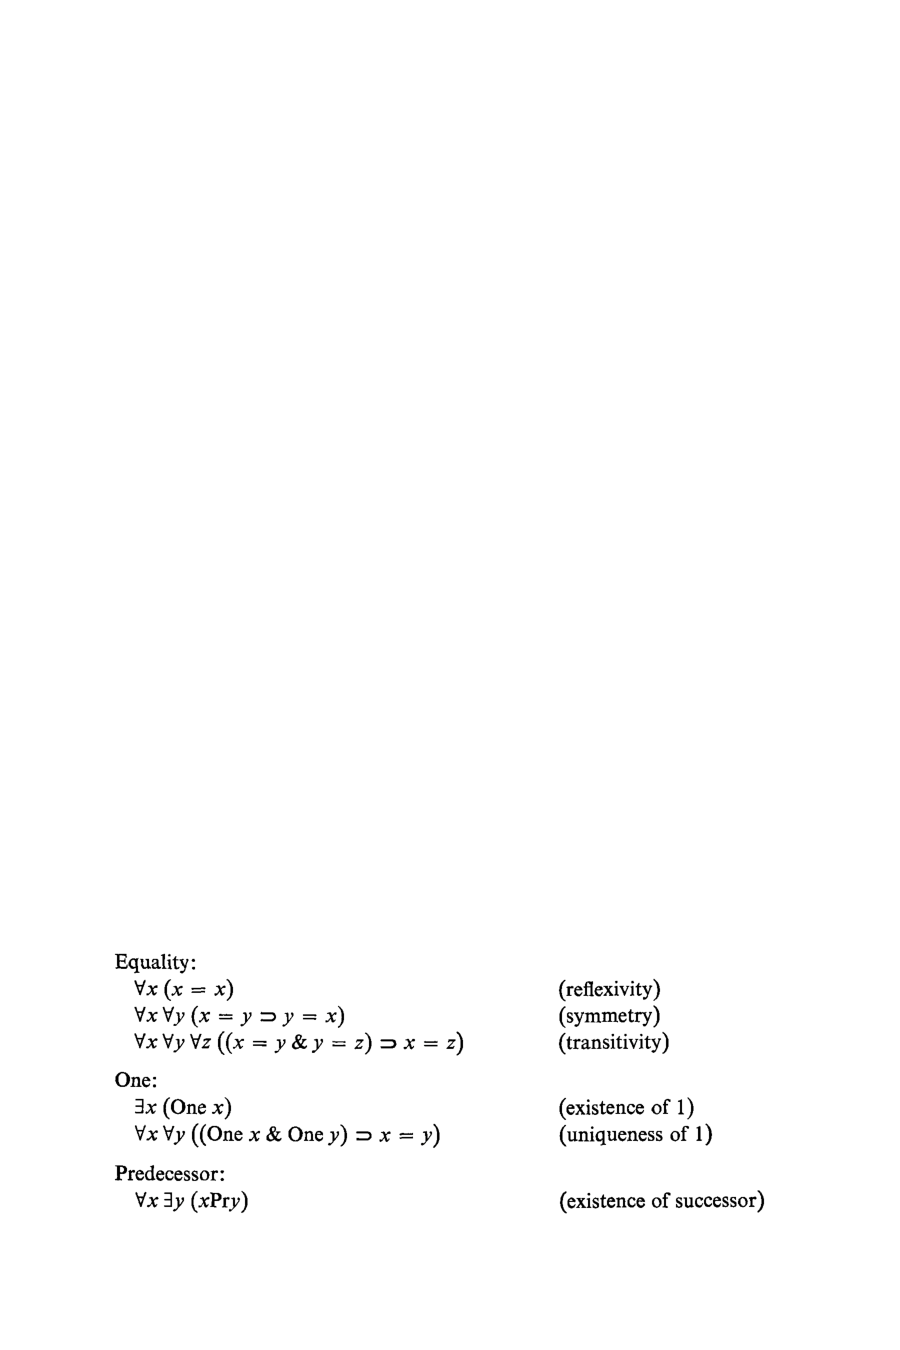
\includegraphics[scale=0.5]{figs/gentzen1} &\qquad& 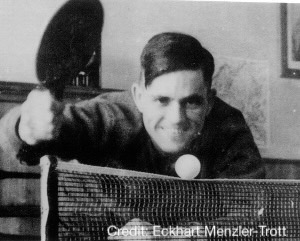
\includegraphics[scale=0.3]{figs/gentzen3}\\
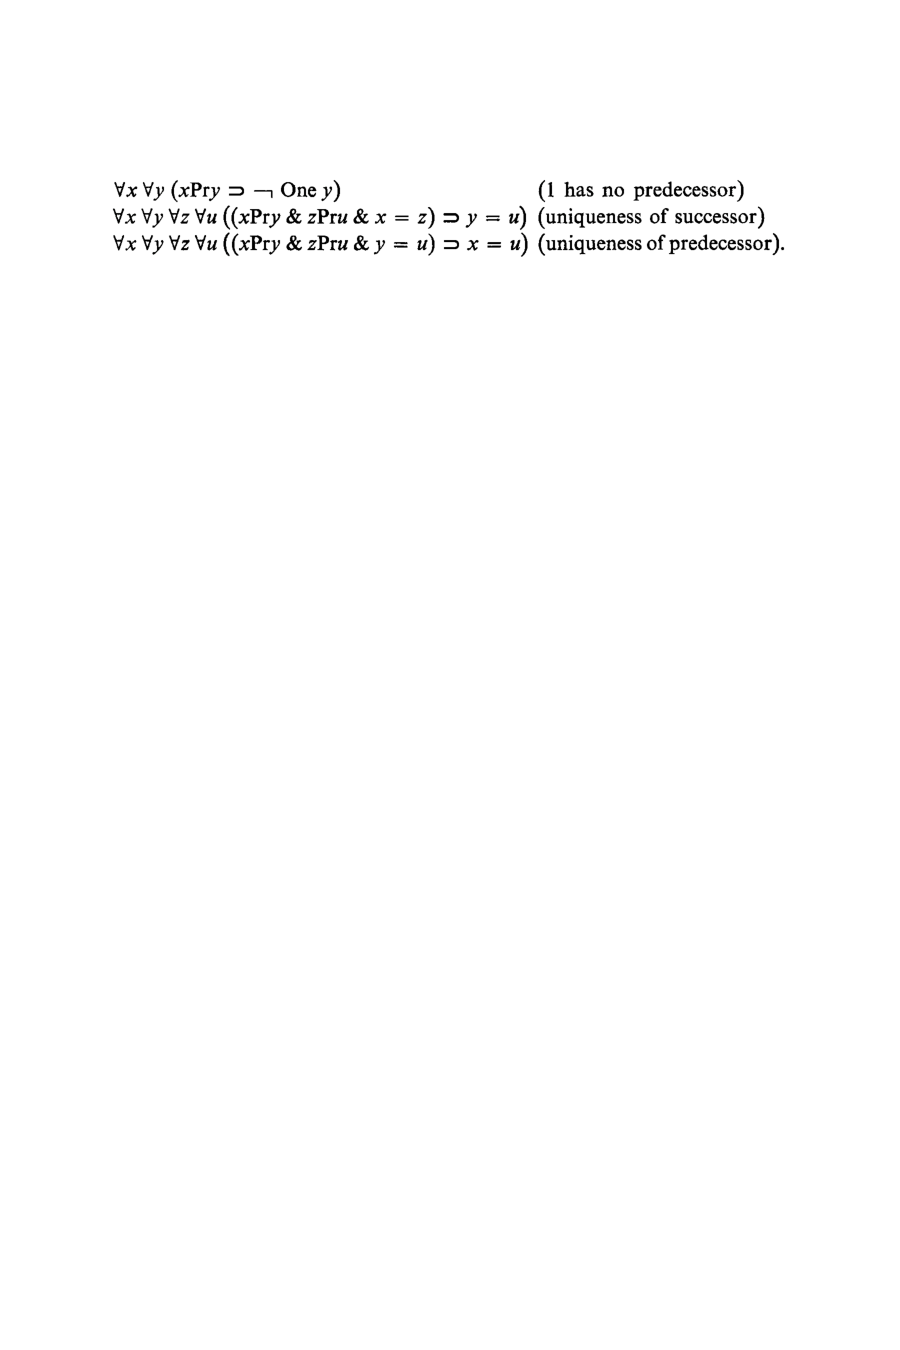
\includegraphics[scale=0.5]{figs/gentzen2} 
\end{tabular}
}	
\only<3>{
\begin{center}
{\em ``If our arithmetic is inconsistent, there exists a [cut-free] $\LK$ derivation with endsequent
\[
\mathfrak{U}_1,\ldots \mathfrak{U}_n\seq
\] 
where $\mathfrak{U}_1,\ldots \mathfrak{U}_n$ are arithmetic axiom formulae.''}
\end{center}
}


\only<4-5>{
\medskip

\emphdo{A naive attempt:} Add non-logical axioms.

\medskip

Assume $\vdash P\impl Q$ and $\vdash P$. 
			Then\semiproofadjust
			$$
			\infer[cut]{\vdash Q}
			{\infer{\vdash P}{}&
				\infer[cut]{P\vdash Q}
				{\infer{\vdash P\impl Q}{}&
					\infer[\impl_l]{P,P\impl Q\vdash Q}
					{\infer{P\vdash P}{}&
						\infer{Q\vdash Q}{}}}}
			$$
}
\only<5>{
\medskip

\emphdb{Girard}: The {\em Hauptsatz} fails for systems with proper axioms.}

\only<6-7>{
\medskip

\emphdo{A better solution:} Add non-logical rules of inference


\medskip
			
			$$
			\infer[\emphdb{P\impl Q}]{\Gamma, P\seq C}{\Gamma, Q\seq C}\qquad
			\infer[\emphdb{P}]{\Gamma\seq C}{\Gamma, P\seq C}
			$$
		}	
		
		\only<7>{
						The sequent $\seq Q$ now has the (cut-free) proof\semiproofadjust
			$$
			\infer[\emphdb{P}]{\seq Q}{\infer[\emphdb{P\impl Q}]{P\seq Q}
				{\infer{Q\seq Q}{}}}
			$$
		}
\end{overlayarea}
\end{frame}

\section{Polarisation}
\begin{frame}
\frametitle{Polarities of connectives}

\textbf{First-order classical and intuitionistic language:}
$$A\coloncolonequals P(x) \mid A \wedge A \mid t \mid A \vee A \mid f \mid A \impl A \mid \exists x\, A \mid \forall x\, A$$

\medskip

\textbf{{Polarized connectives:}}
\begin{itemize}
\item In \emphdr{classical  logic}%, the \emph{polarized connectives} are:
\begin{itemize}
\item \posf{positive} and \negf{negative} versions of the logical connectives and constants: 
\[\wedgen, \wedgep, \truen, \truep,\veen, \veep, \falsen, \falsep\]
\item first-order quantifiers: $\forall$ \negf{negative} and $\exists$ \posf{positive}.
\end{itemize}
\item In \emphdr{intuitionistic logic} 
\begin{itemize}
\item polarized classical connectives and constants where $\falsen,\veen$ do not occur;
\item \negf{negative} implication: $\impl$.
\end{itemize}
\item A formula is \posf{positive} if it is a positive atom or has a
top-level positive connective.
\item A formula is \negf{negative} if it is a
negative atom or has a top-level negative connective.
\end{itemize}
\end{frame}


\begin{frame}{A fresh view to an old problem}

\begin{overlayarea}{\textwidth}{7cm}			
		
		\only<1->{
			Combining the classification of axioms into a \emphdb{polarities' hierarchy} [Ciabattoni et al.]
}
\only<1>{	
			\medskip
		

\begin{center}
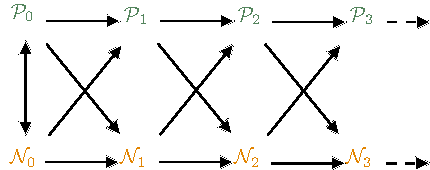
\includegraphics[scale=0.8]{figs/h5}
\end{center}
}
\only<1>{
\medskip 
{\small $(\forall x\posf{P_1}\wedgen\posf{P_2})\wedgen(\forall y{B(y)}\wedgen \posf{P_3})$}
	\parbox[c]{2.5cm}{
		\scalebox{.65}{
			\begin{tikzpicture}[sibling distance=7em,level distance=4ex, level 2/.style={sibling distance =4em}]
			\node (neg 1) {$\wedgen$\strut}
			child { node {\rlap{$\wedgen$}\phantom{$\vee$}}
				child { node {$\forall$}
					child[level distance=3ex] {node[itria] {\smash{\posf{$P_1$}}}}}
				child {
					child[level distance=1ex] {node[itria] {\smash{\posf{$P_2$}}}}}}
			child { node {\rlap{$\wedgen$}\phantom{$\vee$}}
				child { node {$\forall$}
					child[level distance=5.5ex] {node {${B(y)}$}}}
				child {
					child[level distance=1ex] {node[itria] {\smash{\posf{$P_3$}}}}}};
			\end{tikzpicture}}}
%
	$\bm\rightarrow$
%
		\parbox[c]{2.5cm}{
		\scalebox{.65}{
			\begin{tikzpicture}[sibling distance=4em,level distance=3.2ex]
			\node[ellipse,draw = orange,fill = orange!10] (neg2) {\negf{$\mathsf{neg}$}}
			child {
				child [level distance=-1ex]{node[itria] {\smash{\posf{$P_1$}}}}}
			child {
				child [level distance=-1ex]{node[itria] {\smash{\posf{$P_2$}}}}}
			child [level distance=6ex]{node {{$B(y)$}}}
			child {
				child [level distance=-1ex]{node[itria] {\smash{\posf{$P_3$}}}}};
			\end{tikzpicture}}}
			
\medskip

\begin{center}
\emphdr{Bipolar} = $\mathcal{N}_2$\\
(polarities flip at most twice)
\end{center}
}

\only<2->{

\medskip

			with a systematic construction of inference rules from axioms using \emphdo{focusing} [Andreoli],
		}
\only<2>{

\medskip

		\begin{tikzpicture}
		\node at (-1.9,2.5) {$\jUnf{\Gamma_1}{\cdot}{\cdot}{\Delta_1}  \quad\ldots\quad \jUnf{\Gamma_n}{\cdot}{\cdot}{\Delta_n}$};
		\node at (-1.5,-1.4) {$\infer[\kern -2pt D_l]{
				\jUnf{\Gamma,B}{\cdot}{\cdot}{\Delta}}{
				\jLf{\Gamma,B}{B}{\Delta}}$};
		
		\node at (0,0) {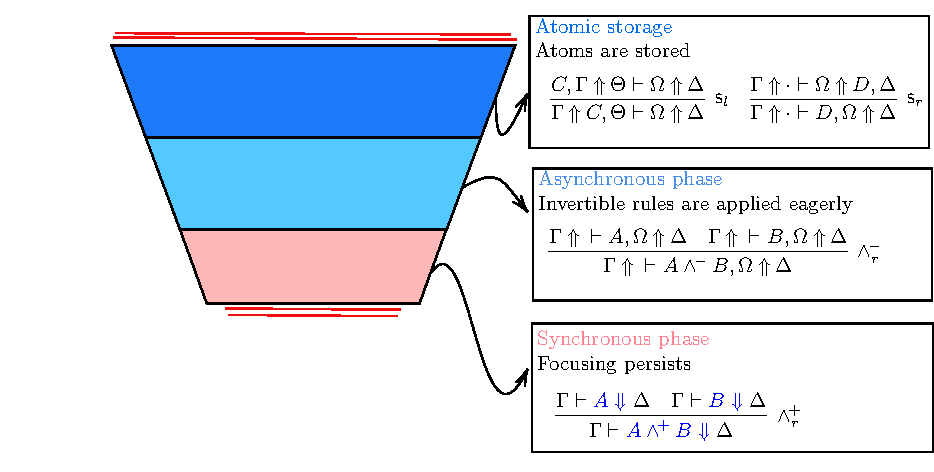
\includegraphics[scale=0.65]{figs/focusing}};
		
		\end{tikzpicture}
}
\only<3->{

\medskip

\emph{justifies} the introduction of the class of \emphdr{bipolar axioms}.}
\only<3>{

\medskip

\begin{tikzpicture}
		\node at (-1.9,2.5) {$\jUnf{\Gamma_1}{\cdot}{\cdot}{\Delta_1}  \quad\ldots\quad \jUnf{\Gamma_n}{\cdot}{\cdot}{\Delta_n}$};
		\node at (-1.5,-1.4) {$\infer[\kern -2pt D_l]{
				\jUnf{\Gamma,B}{\cdot}{\cdot}{\Delta}}{
				\jLf{\Gamma,B}{B}{\Delta}}$};
				
\node at (-2.2,0.7) {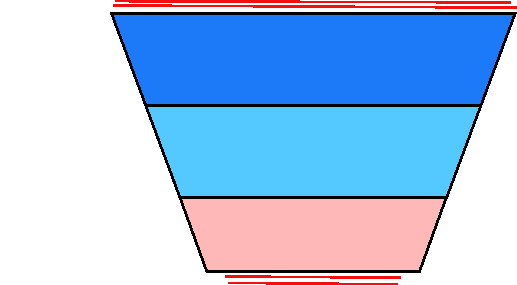
\includegraphics[scale=0.65]{figs/focusing2}};
		%
		\node at (4,1) {\textbf{Corresponding synthetic rule}};
		\node at (4,0.5) {(in $\LK$ or $\LJ$)};
		\node at (4,-0.5) {
			$\infer{\Gamma \seq \Delta}{\Gamma_1 \seq \Delta_1 \quad\ldots\quad \Gamma_n\seq\Delta_n}$};
			\end{tikzpicture}
			}
\end{overlayarea}
\end{frame}

\begin{frame}\frametitle{The main results [Marin, Miller, Pimentel \& Volpe]}	
	
	\begin{block}{}
		\textbf{Theorem 1.} 
		Bipolar axioms correspond to sequent inference rules.
	\end{block}
	
	\bigskip
	
	\begin{block}{}
		\textbf{Theorem 2.} 
		The cut rule is admissible in the extension of $\LK/\LJ$ with the  inference rules
corresponding to bipolar axioms.
	\end{block}


\end{frame}

%\section{The roadmap}
%
%\begin{frame}\frametitle{Obtaining rules from axioms}
%	
%	\scalebox{.8}{
%		\begin{tikzpicture}
%		\tikzstyle{operation}=[->,>=latex,thick]
%		\tikzstyle{state}=[rectangle,draw,thick, rounded corners=5pt, text width = 1.6cm, align=center]
%		\tikzstyle{etiquette}=[rectangle,draw,thick,dotted]
%		%%rectangles
%		%\draw [fill=red!20, thick] (5,-0.5) rectangle (8,-3.5);
%		%\draw [fill=blue!20, thick, rounded corners=7pt] (-1.5,-0.5) rectangle (1.5,0.5);
%		%%points
%		\uncover<1->{
%			\node[state, fill=gray!20] (i) at (0,0)  {Unpolarized\\Axiom};
%		}
%		\only<1,12>{
%			\node[right = of i] {$\forall x (((P_1(x) \impl P_2(x)) \wedge Q(x)) \impl\exists y R(x,y))$};
%		}
%		%
%		\uncover<2->{
%			\node[state, fill=blue!20] (ii) at (2.5,2) {Polarized\\Axiom};
%			\node[state, fill=blue!20] (ii') at (2.5,-2) {Polarized\\Axiom};
%			%	\draw[dotted,thick] (2.5,1.2)--(2.5,-1.2);
%		}
%		%
%		\uncover<2->{
%			\draw[operation] (i)--(ii) node[etiquette] at (0.7,1.2) {Polarizing};
%			\draw[operation] (i)--(ii');
%		}
%		\only<2-5,9,11>{
%			\draw[operation,dotted] (i)--(2,0.8);
%			\draw[operation,dotted] (i)--(2,0);
%			\draw[operation,dotted] (i)--(2,-0.8);
%		}
%		%
%		\only<2-4>{
%			\node[right] at (2,0.8) {$\negf{\bm\forall}x (((\posf{P_1}(x) \negf{\bm\impl} \negf{P_2}(x)) \posf{\bm\wedgep} \posf{Q}(x)) \negf{\bm\impl}\posf{\bm\exists}y \posf{R}(x,y))$};
%		}
%		\only<2-3,9>{
%			\node[right] at (2,0) {$\negf{\bm\forall}x (((\posf{P_1}(x) \negf{\bm\impl} \negf{P_2}(x)) \negf{\bm\wedgen} \negf{Q}(x)) \negf{\bm\impl}\posf{\bm\exists}y \posf{R}(x,y))$};
%		}
%		\only<2-3,11>{
%			\node[right] at (2,-0.8) {$\negf{\bm\forall}x (((\posf{P_1}(x) \negf{\bm\impl} \negf{P_2}(x)) \negf{\bm\wedgen} \posf{Q}(x)) \negf{\bm\impl}\posf{\bm\exists}y \posf{R}(x,y))$};
%		}
%		%
%		\uncover<3->{
%			\node[etiquette] at (4.5,3) {Is it bipolar?};
%		}
%		%
%		\uncover<4-8,9-10,12>{
%			\draw[thick] (ii)--(4.5,2) node[circle,draw,fill=green!40] {$\bm\checkmark$};
%		}
%		\uncover<11-12>{
%			\draw[thick] (ii')--(4.5,-2) node[circle,draw,fill=red!40] {$\bm\times$};%node[etiquette] 
%		}
%		%
%		\uncover<5-8,10,12>{
%			\node[state, fill=green!20] (iii) at (6.5,2) {Bipole\\in \LKF}; 
%			\draw[operation] (4.85,2)--(iii);
%		}
%		\only<5-7>{
%			\node[] at (8.5,-0.5) {$
%				\infer[\forall_l]{\jLf{\Gamma}{\negf{\bm\forall}x (((\posf{P_1}(x) \negf{\bm\impl} \negf{P_2}(x)) \posf{\bm\wedgep} \posf{Q}(x)) \negf{\bm\impl}\posf{\bm\exists}y \posf{R}(x,y))}{}{\Delta}}{
%					\infer[\impl_l]{{\jLf{\Gamma}{((P_1(t) \impl P_2(t)) \wedgep Q(t)) \impl \exists y R(t,y)}{}{\Delta}}}{
%						\infer[\wedgep_r]{\jRf{\Gamma}{(P_1(t) \impl P_2(t)) \wedgep Q(t)}{\Delta}}{
%							\infer[\krelease_r]{{\jRf{\Gamma}{P_1(t)\impl P_2(t)}{\Delta}}}{
%								\infer[\impl_r]{\jUnf{\Gamma}{\cdot}{P_1(t)\impl P_2(t)}{\Delta}}{
%									\infer[\kstore_l]{\jUnf{\Gamma}{P_1(t)}{P_2(t)}{\Delta}}{
%										\infer[\kstore_r]{\jUnf{\Gamma,P_1(t)}{\cdot}{P_2(t)}{\Delta}}{
%											\deduce{\jUnf{\Gamma,\posf{P_1(t)}}{\cdot}{\cdot}{\negf{P_2(t)},\Delta}}{}
%										}
%									}
%								}
%							} 
%							& 
%							\infer[\kinit_r]{\jRf{\Gamma}{\posf{Q(t)}}{\Delta}}{}
%						} 
%						& 
%						\infer[\krelease_l]{\jLf{\Gamma}{\exists y R(t,y)}{\Delta}}{
%							\infer[\exists_l]{\jUnf{\Gamma}{\exists y R(t,y)}{\cdot}{\Delta}}{
%								\infer[\kstore_l]{\jUnf{\Gamma}{R(t,z)}{\cdot}{\Delta}}{
%									\deduce{\jUnf{\Gamma, \posf{R(t,z)}}{\cdot}{\cdot}{\Delta}}{}
%								}
%							}
%						}
%					}
%				}
%				$};
%		}
%		%
%		\uncover<7-12>{
%			\node[state, fill=orange!20] (iv) at (9.5,2) {Inference\\rule for \LK};
%		}
%		\uncover<6-8,12>{
%			\draw[operation] (iii)--(iv) node[etiquette] at (8,3) {Synthesizing};
%		}
%		\only<7-8>{
%			\node[draw] at (11,1) {$
%				\infer[]{\Gamma = \Gamma', \emphdr{Q(t)}\seq\Delta}{
%					\Gamma, \emphdr{P_1(t)}\seq\emphdr{P_2(t)},\Delta
%					& 
%					\Gamma, \emphdr{R(t,z)}\seq\Delta}
%				$};
%		}
%		%
%		\only<10>{
%			\node[draw] at (10.5,1) {$
%				\infer[]{\Gamma\seq\Delta}{
%					\Gamma, \emphdr{P_1(t)}\seq\emphdr{P_2(t)},\Delta
%					&
%					\Gamma \seq\emphdr{Q(t)},\Delta
%					& 
%					\Gamma, \emphdr{R(t,z)}\seq\Delta}
%				$};
%		}
%		%
%		\only<12>{
%			\node[draw] at (11.5,0) {$
%				\infer[]{\Gamma = \Gamma', \emphdr{Q(t)}\seq\Delta}{
%					\Gamma, \emphdr{P_1(t)}\seq\emphdr{P_2(t)},\Delta
%					& 
%					\Gamma, \emphdr{R(t,z)}\seq\Delta}
%				$};
%			\node[draw] at (10.5,-1.5) {$
%				\infer[]{\Gamma\seq\Delta}{
%					\Gamma, \emphdr{P_1(t)}\seq\emphdr{P_2(t)},\Delta
%					&
%					\Gamma \seq\emphdr{Q(t)},\Delta
%					& 
%					\Gamma, \emphdr{R(t,z)}\seq\Delta}
%				$};
%		}
%		\end{tikzpicture}
%	}
%	
%	
%\end{frame}





\section{Examples}
%\subsection{Geometric axioms}
%
%\begin{frame}\frametitle{Geometric axioms as bipoles}
%	
%\only<1>{\emphdr{Geometric implication:}}
%%
%\only<2->{\emphdo{Polarized geometric implication:}}
%		
%%\begin{overlayarea}{\textwidth}{1cm}
%\only<1>{
%		\[\forall \overline{z} (P_1 \wedge \ldots \wedge P_m \, \impl \, \exists \overline{x}_1 M_1 \vee \ldots \vee \exists \overline{x}_n M_n ) 
%		\]
%}	
%\only<2>{
%\[\negf{\forall \overline{z}} (P_1^{\pm} \wedgepn \ldots \wedgepn P_m^{\pm} \, \negf{\impl} \, \posf{\exists \overline{x}_1} \hat{M_1} \veepn \ldots \veepn \posf{\exists \overline{x}_n} \hat{M_n} )
%		\]
%}
%\only<3>{
%	$$
%	\negf{\forall \overline{z}} (\posf{P_1^{+}} \posf{\wedgep} \ldots \posf{\wedgep} \posf{P_m^{+}} \, \negf{\impl} \, \posf{\exists \overline{x}_1} \hat{M_1} \veepn \ldots \veepn \posf{\exists \overline{x}_n} \hat{M_n} ) \, ,
%	$$
%}
%\only<4>{
%	$$
%	\negf{\forall \overline{z}} (\negf{P_1^{-}} \wedgepn \ldots \wedgepn \negf{P_m^{-}} \, \negf{\impl} \, \posf{\exists \overline{x}_1} \hat{M_1} \veepn \ldots \veepn \posf{\exists \overline{x}_n} \hat{M_n} ) \, ,
%	$$
%}
%%\end{overlayarea}
%
%\bigskip
%
%\begin{overlayarea}{\textwidth}{4cm}
%\only<1>{
%\begin{itemize}
%	\item $P_i$ atomic;
%	\item $M_j=Q_{j_1}\wedge\ldots\wedge Q_{j_{k_{j}}}$, $Q_{j_k}$ atomic; 
%	\item none of the variables in the vectors $\overline{x}_j$ are free in $P_i$.
%\end{itemize}	
%}
%\only<2>{
%\begin{itemize}
%\item $\posf{P_i^+}, \negf{P_i^-}$ atomic;
%\item $\hat{M_j} = Q_{j_1}^{\pm} \posf{\wedgep} \ldots \posf{\wedgep} Q_{j_{k_{j}}}^{\pm}$ , $Q_{j_k}^{\pm}$ atomic;
%\item none of the variables in the vectors $\overline{x}_j$ are free in $P_i$.
%\end{itemize}
%}		
%\only<3>{
%		\emph{Corresponding bipole}:	
%		$$\infer{\jUnf{\emphdr{\overline{P}},\Gamma'}{\null}{\null}{\Delta}}
%		{\jUnf{\emphdr{\overline{Q}_1[\overline{y}_1/\overline{x}_1]},\Gamma}{\null} {\null}{\Delta} & \ldots & \jUnf{\emphdr{\overline{Q}_n[\overline{y}_n/\overline{x}_n]},\Gamma}{\null} {\null}  {\Delta}}
%		$$
%		with $\overline{P}=\{\posf{P_i^+}\}, \overline{Q_j}=\{Q_{j_k}^\pm\}$. 
%
%		\bigskip
%				
%		\emphdb{Corresponding $\LK$ rule}:	
%		$$\infer[GRS]{\emphdr{\overline{P}},\Gamma'\vdash \Delta}
%		{\emphdr{\overline{Q}_1[\overline{y}_1/\overline{x}_1]},\Gamma\vdash\Delta & \ldots & \emphdr{\overline{Q}_n[\overline{y}_n/\overline{x}_n]},\Gamma\vdash\Delta}
%		$$
%	}
%	
%	\only<4>{
%		\emph{Corresponding bipole}:	
%		$$\infer[m+n\mbox{ premises}]{\jUnf{\Gamma}{\null}{\null}{\Delta}}
%		{\jUnf{\emphdr{\overline{Q}_j[\overline{y}_j/\overline{x}_j]},\Gamma}{\null} {\null}{\Delta} & \ldots &\jUnf{\Gamma}{\null} {\null}{\emphdr{P_i},\Delta} }
%		$$
%with $\overline{Q_j}=\{Q_{j_k}\}$. 
%
%		\bigskip
%				
%		\emphdb{Corresponding $\LK$ rule}:	
%		$$\infer[m+n\mbox{ premises}]{\Gamma\vdash \Delta}
%		{\emphdr{\overline{Q}_j[\overline{y}_j/\overline{x}_j]},\Gamma\vdash \Delta & \ldots & \Gamma\vdash \emphdr{P_i},\Delta}
%		$$		
%		}
%\end{overlayarea}
%	
%\end{frame}


\begin{frame}\frametitle{\only<1-4>{Example: Horn clauses as bipoles} \only<5>{Other examples}}

\only<1>{\[
		\forall \overline{z}(P_1 \wedge \ldots \wedge P_m \, \impl \, Q)
		\]}
	
\only<2>{\[
		\negf{\forall \overline{z}}(P_1^{\pm} \wedgepn \ldots \wedgepn P_m^{\pm} \, \negf{\impl} \, Q^{\pm})
		\]}
	
\only<3>{\[
	\negf{\forall \overline{z}}(\posf{P_1^{+}} \posf{\wedgep} \ldots \posf{\wedgep} \posf{P_m^{+}} \, \negf{\impl} \, \posf{Q^{+}} )
	\]}

\only<4>{\[
	\negf{\forall \overline{z}}(\negf{P_1^{-} \wedgen} \ldots \negf{\wedgen P_m^{-}} \, \negf{\impl} \, \negf{Q^{-}})
	\]}
		
\bigskip


\begin{overlayarea}{\textwidth}{2cm}
\only<3>{
$$	\infer[FC]
	{\emphdr{\overline{P}}, \Gamma'\vdash\Delta}
	{\emphdr{Q}, \Gamma\vdash\Delta}	
	$$
\begin{center}
\emph{Forward-chaining} \\
\emph{[Simpson, Negri, Ciabattoni]}
\end{center}
}

\only<4>{
$$\infer[BC]
	{\Gamma\vdash \emphdr{Q},\Delta'}
	{\Gamma\vdash \emphdr{P_1}, \Delta & \ldots &\Gamma\vdash \emphdr{P_m}, \Delta}
	$$
\begin{center}
\emph{Back-chaining}\\
\emph{[Vigan\`o]}
\end{center}
}
\only<5>{
\begin{center}
Geometric, co-geometric, universal axioms...
\end{center}
\medskip
\[\negf{\forall \overline{z}} (P_1^{\pm} \wedgepn \ldots \wedgepn P_m^{\pm} \, \negf{\impl} \, \posf{\exists \overline{x}_1} \hat{M_1} \veepn \ldots \veepn \posf{\exists \overline{x}_n} \hat{M_n} )
		\]
		\smallskip
\[
		\negf{\forall \overline{z}} (\negf{\forall \overline{x}_1} \hat{M_1} \wedgepn \ldots \wedgepn \negf{\forall \overline{x}_n} \hat{M_n}  \, \negf{\impl} \, \negf{P_1^{-} \veen} \ldots \negf{\veen P_m^{-}} ) 
		\]
		\smallskip
\[
		\negf{\forall \overline{z}}(P_1^{\pm} \wedgepn \ldots \wedgepn P_m^{\pm} \, \negf{\impl} \, Q_1^{\pm} \veepn \ldots \veepn Q_n^{\pm})
		\]
}
\end{overlayarea}
\end{frame}




\end{document}
